\exercise{Lista Doppiamente Collegata}
Si realizzi in linguaggio C++ il tipo di dato astratto \cod{Lista} mediante uso del costrutto \cod{class} del linguaggio. L'implementazione deve essere realizzata mediante puntatori ed allocazione dinamica della memoria secondo l'approccio di lista doppiamente collegata. Ogni elemento, cio�, punta contemporaneamente al precedente ed al successivo (vedi \figurename~\ref{fig:ListaDoppiamenteCollegata}). Gli elementi della lista siano di tipo \cod{TElem} uguale al tipo \cod{int}.

\begin{figure}
  \center
	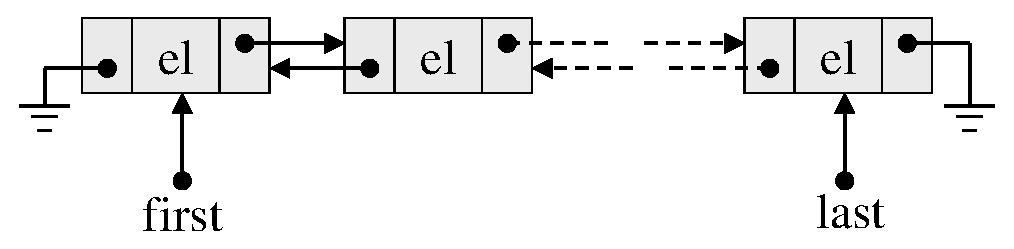
\includegraphics[width=.7\textwidth]{Esercizi/ListaDoppiamenteCollegata/Lista.eps}
	\caption{Struttura della lista doppiamente collegata}
	\label{fig:ListaDoppiamenteCollegata}
\end{figure}
        
Di seguito � riportata la specifica dei metodi pubblici da implementare per la classe \cod{Lista}.

\begin{methodslist}

\method{Lista}{\emptyset}{\emptyset} {
Costruttore.
}

\method{\~{}Lista}{\emptyset}{\emptyset} {
Distruttore.
}

\method{Inserisci}{TElem}{\emptyset} {
Inserisce un elemento in coda alla lista.
}

\method{Svuota}{\emptyset}{\emptyset} {
Svuota la lista.
}

\method{Count}{\emptyset}{unsigned int} {
Conta gli elementi contenuti nella lista.
}

\method{StampaDiretta}{\emptyset}{\emptyset} {
Stampa il contenuto della lista sullo standard output, dall'elemento di testa all'elemento di coda.
}

\method{StampaInversa}{\emptyset}{\emptyset} {
Stampa il contenuto della lista sullo standard output, dall'elemento di coda all'elemento di testa.
}

\method{StampaAlternata}{\emptyset}{\emptyset} {
Stampa il contenuto della lista nel seguente ordine: primo elemento, ultimo elemento, secondo elemento, penultimo elemento, terzo elemento, terzultimo elemento...
}

Gli unici metodi della classe Lista che possono utilizzare lo standard-output (\cod{cout}) sono i metodi di stampa. Gli altri metodi (pubblici, privati o protetti) non possono fare uso degli oggetti per l'I/O.

Si realizzi una funzione \cod{main()} che permetta di effettuare il collaudo della struttura dati realizzata.

\end{methodslist}